%!TEX root = ../../../adrien_gomar_phd.tex


\begin{figure}[htb]
  \centering
  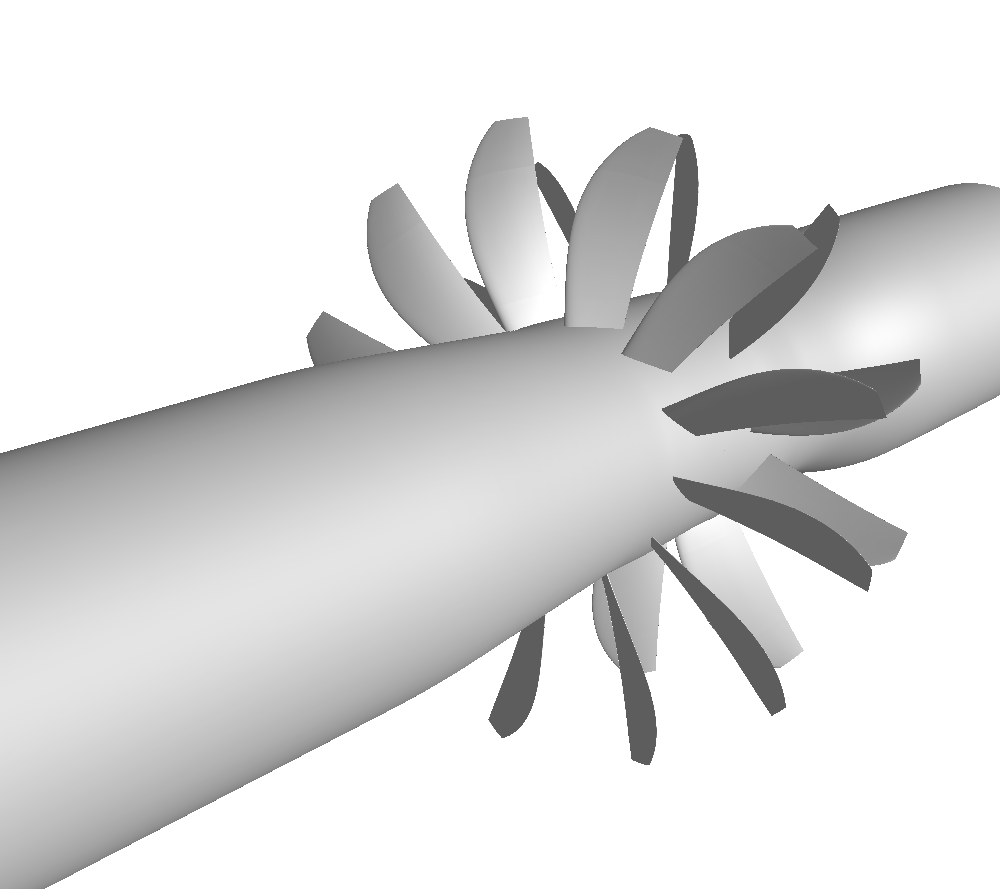
\includegraphics[width=.3\textwidth]{DREAM_LS_wall.png}
  \caption{Low-speed isolated contra-rotating open rotor geometry.}
  \label{fig:dream_ls_wall}
\end{figure}

The DREAM configuration is a pusher contra-rotating open rotor.
It is shown in Fig.~\ref{fig:dream_ls_wall} for the
Low-speed (LS) or take-off flight condition. 
The simulated configuration does not include the spinner as the
experimental setup does not include this part of the geometry.
Sadly, the experimental results were not available for comparison
at the time this PhD thesis has been written.

\begin{table}[htb]
  \ra{1.3} \centering
  \begin{tabular}{cccc}
    \toprule
    $M_0$ & $|\Omega|$ & $J$ & $M_{tip}$ \\
    \midrule
    $0.2$ & $5739$ tr.min\textsuperscript{-1} & 1.06 & 0.63 \\
    \bottomrule
  \end{tabular}
  \caption{Low-speed isolated contra-rotating open rotor flight condition parameters.}
  \label{tab:dream_ls_flight_condition}
\end{table} 
Table~\ref{tab:dream_ls_flight_condition} recalls the main
parameters of the case: the inlet Mach number $M_0$,
the absolute value of the rotation speed of both rotors $|\Omega|$,
the advance ratio $J$ (whose definition is given in Chap.~\ref{cha:cror})
and the Mach number at the tip of
the blade based on the inlet velocity and the advance ratio:
\begin{equation}
	M_{tip} = M_0 \sqrt{1 + \left(\frac{\pi}{J} \right)^2}
\end{equation}
This equation is a simple transcription of the velocity triangle
applied to the infinite velocity and to the rotation speed perceived
at the front blade tip:
\begin{equation}
    M_{tip} = M_0 \sqrt{1 + \left(\frac{\pi}{J}\right)^2} = 
    \frac{V_0}{\sqrt{\gamma R T_0}} \sqrt{1 + \left(\frac{
    	\cancel{\pi} \cdot \Omega D}{
    	2 \cancel{\pi} \cdot V_0}\right)^2} =
    \sqrt{\frac{V_0^2 + (\Omega R)^2}{\gamma R T_0}}
    \label{eq:m_tip_explained}
\end{equation}
